%%%%%%%%%%%%%%%%%%%%%%%%%%%%%%%%%%%%%%%%%%%%%%%%%%%%%%%%%%%%%%%%%%%%%%%%%%%%%%%%%
%%%%%%%%%%%%%%%%%%%%%%%%%%%%%%%%%%%%%%%%%%%%%%%%%%%%%%%%%%%%%%%%%%%%%%%%%%%%%%%%%
%%%%%%%%%%%%%%%%%%%%%%%%%%%%%%%%%%%%%%%%%%%%%%%%%%%%%%%%%%%%%%%%%%%%%%%%%%%%%%%%%
%%% TODO

% Define pre-handouts



%%%%%%%%%%%%%%%%%%%%%%%%%%%%%%%%%%%%%%%%%%%%%%%%%%%%%%%%%%%%%%%%%%%%%%%%%%%%%%%%%
%%%%%%%%%%%%%%%%%%%%%%%%%%%%%%%%%%%%%%%%%%%%%%%%%%%%%%%%%%%%%%%%%%%%%%%%%%%%%%%%%
%%%%%%%%%%%%%%%%%%%%%%%%%%%%%%%%%%%%%%%%%%%%%%%%%%%%%%%%%%%%%%%%%%%%%%%%%%%%%%%%%
%%% packages

\usepackage[english]{babel}
\usepackage{amsmath, amssymb}
\usepackage{array} 
\usepackage{tikz}
\usetikzlibrary{backgrounds}
%\usepackage{slashbox}
%\usepackage{pict2e}
%\usetikzlibrary{backgrounds}
%\usetikzlibrary{matrix}
\usepackage{url}
\usepackage{hyperref}
\usepackage{colordvi}
%\usepackage{xcolor, colortbl}
\usepackage{enumerate}
\usepackage[round]{natbib}
\usepackage{ifthen}
\usepackage{rotating}
\usepackage{varwidth}



%%%%%%%%%%%%%%%%%%%%%%%%%%%%%%%%%%%%%%%%%%%%%%%%%%%%%%%%%%%%%%%%%%%%%%%%%%%%%%%%%
%%%%%%%%%%%%%%%%%%%%%%%%%%%%%%%%%%%%%%%%%%%%%%%%%%%%%%%%%%%%%%%%%%%%%%%%%%%%%%%%%
%%%%%%%%%%%%%%%%%%%%%%%%%%%%%%%%%%%%%%%%%%%%%%%%%%%%%%%%%%%%%%%%%%%%%%%%%%%%%%%%%
%%% beamer settings

\usetheme{Frankfurt}

\useoutertheme[subsection=false]{smoothbars}
\useinnertheme[shadow=true]{rounded}

\usecolortheme{orchid}
\usecolortheme{whale}

\setbeamertemplate{navigation symbols}{}

\setbeamertemplate{footline}[text line]{\color{dkgreen} \bf
  \insertshortauthor \hfill \insertshorttitle \hfill 15th Reasoning
  Web Summer School (RW
  2019) \hfill \insertframenumber/\inserttotalframenumber}

\setbeamersize{text margin left=0.5cm} 
\setbeamersize{text margin right=0.5cm} 



%%%%%%%%%%%%%%%%%%%%%%%%%%%%%%%%%%%%%%%%%%%%%%%%%%%%%%%%%%%%%%%%%%%%%%%%%%%%%%%%%
%%%%%%%%%%%%%%%%%%%%%%%%%%%%%%%%%%%%%%%%%%%%%%%%%%%%%%%%%%%%%%%%%%%%%%%%%%%%%%%%%
%%%%%%%%%%%%%%%%%%%%%%%%%%%%%%%%%%%%%%%%%%%%%%%%%%%%%%%%%%%%%%%%%%%%%%%%%%%%%%%%%
%%% commands

%%%%%%%%%%%%%%%%%%%%%%%%%%%%%%%%%%%%%%%%%%%%%%%%%%%%%%%%%%%%%%%%%%%%%%%%%%%%%%%%%
%%%%%%%%%%%%%%%%%%%%%%%%%%%%%%%%%%%%%%%%%%%%%%%%%%%%%%%%%%%%%%%%%%%%%%%%%%%%%%%%%
%%%%%%%%%%%%%%%%%%%%%%%%%%%%%%%%%%%%%%%%%%%%%%%%%%%%%%%%%%%%%%%%%%%%%%%%%%%%%%%%%
%%% slides stuff

\newcommand{\blocknode}[5]{\node (#1) at #2 {%
    \begin{minipage}{3.5cm}\begin{block}{#4}
        \begin{overlayarea}{3.5cm}{#3}
        #5\end{overlayarea}\end{block}\end{minipage}};}
\newcommand{\smallblocknode}[5]{\node (#1) at #2 {%
    \begin{minipage}{3.0cm}\begin{block}{#4} \begin{overlayarea}{3.0cm}{#3}
    #5\end{overlayarea}\end{block}\end{minipage}};}
\newcommand{\redsmallblocknode}[5]{\node (#1) at #2 {%
    \begin{minipage}{3.0cm}\begin{alertblock}{#4} \begin{overlayarea}{3.0cm}{#3}
    #5\end{overlayarea}\end{alertblock}\end{minipage}};}



\renewcommand{\newblock}{}
\definecolor{ToDoColor}{rgb}{0,0.16,0.90} %blue
\definecolor{OutlineColor}{rgb}{0.2,0.8,0.2} %green
\definecolor{CommentColor}{rgb}{0.90,0.16,0} %red
\definecolor{dkgreen}{rgb}{0,0.5,0}
\definecolor{mLightBrown}{rgb}{0.71,0.40,0.11}
\definecolor{mLightGreen}{rgb}{0.56,0.93,0.56}
\newcommand<>{\textblue}[1]{{\color#2{blue}#1}}
\newcommand<>{\textred}[1]{{\color#2{red}#1}}
\newcommand<>{\textgreen}[1]{{\color#2{green}#1}}
\newcommand<>{\textdkgreen}[1]{{\color#2{dkgreen}#1}}
\newcommand<>{\textorange}[1]{{\color#2{orange}#1}}
\newcommand<>{\textyellow}[1]{{\color#2{yellow}#1}}

\newcommand{\ie}{i.\,e.}
\newcommand{\eg}{e.\,g.}
\newcommand{\cf}{cf.}

\newcommand{\notesym}{\ensuremath{\to}} 
\newcommand{\noteblk}[1]{
\begin{block}{}
#1
\end{block}} 

\newcommand{\lectureslides}[1]{\ifthenelse{\value{VERSION}=0}{#1}{}}
\newcommand{\nolectureslides}[1]{\ifthenelse{\not\value{VERSION}=0}{#1}{}}
\newcommand{\posthandout}[1]{\ifthenelse{\value{VERSION}=1}{#1}{}}
\newcommand{\noposthandout}[1]{\ifthenelse{\not\value{VERSION}=1}{#1}{}}
\newcommand{\prehandout}[1]{\ifthenelse{\value{VERSION}=2}{#1}{}}
\newcommand{\noprehandout}[1]{\ifthenelse{\not\value{VERSION}=2}{#1}{}}


\newcommand{\images}{../IMAGES}
\graphicspath{{../IMAGES/}}
\newcommand{\rovergoal}[1]{
\includegraphics[scale=0.06]{rovergoal#1.png}
}


%%%%%%%%%%%%%%%%%%%%%%%%%%%%%%%%%%%%%%%%%%%
%%% defs, propositions, etc

\newenvironment{mydef}[1]{

\begin{block}{#1}
}{
\end{block}
}

\newenvironment{myprop}[1]{

\begin{block}{Proposition (#1)}
}{
\end{block}
}

\newenvironment{myproof}{

\begin{block}{Proof}
}{
\end{block}
}



%%%%%%%%%%%%%%%%%%%%%
%%%
%%% quiz: highlight ``correct'' (green, 2), ``discuss''
%%% (orange, 1), ``false'' (red, 0) in post-handouts only!

\newcommand{\quiz}[9]{

\prehandout{
\begin{block}{Quiz}
\textbf{#1}
\vspace{-0.15cm}
\begin{columns}
\begin{column}{.45\textwidth}
\begin{itemize}
\item[\textblue{(A):}] #2\vspace{-0.05cm}
\item[\textblue{(C):}] #4
\end{itemize}
\end{column}
\begin{column}{.45\textwidth}
\begin{itemize}
\item[\textblue{(B):}] #3\vspace{-0.05cm}
\item[\textblue{(D):}] #5
\end{itemize}
\end{column}
\end{columns}
\end{block}
}

\lectureslides{
\begin{block}{Quiz}
\textbf{#1}
\vspace{-0.15cm}
\begin{columns}
\begin{column}{.45\textwidth}
\begin{itemize}
\item[\textblue{(A):}] #2\vspace{-0.05cm}
\item[\textblue{(C):}] #4
\end{itemize}
\end{column}
\begin{column}{.45\textwidth}
\begin{itemize}
\item[\textblue{(B):}] #3\vspace{-0.05cm}
\item[\textblue{(D):}] #5
\end{itemize}
\end{column}
\end{columns}
\end{block}
}

\posthandout{
\begin{block}{Quiz}
\textbf{#1}
\vspace{-0.15cm}
\begin{columns}
\begin{column}{.45\textwidth}
\begin{itemize}
\item[\textblue{(A):}] \ifthenelse{#6=0}{\textred{#2}}{\ifthenelse{#6=1}{\textorange{#2}}{\ifthenelse{#6=2}{\textdkgreen{#2}}{}}}\vspace{-0.05cm}
\item[\textblue{(C):}] \ifthenelse{#8=0}{\textred{#4}}{\ifthenelse{#8=1}{\textorange{#4}}{\ifthenelse{#8=2}{\textdkgreen{#4}}{}}}
\end{itemize}
\end{column}
\begin{column}{.45\textwidth}
\begin{itemize}
\item[\textblue{(B):}] \ifthenelse{#7=0}{\textred{#3}}{\ifthenelse{#7=1}{\textorange{#3}}{\ifthenelse{#7=2}{\textdkgreen{#3}}{}}}\vspace{-0.05cm}
\item[\textblue{(D):}] \ifthenelse{#9=0}{\textred{#5}}{\ifthenelse{#9=1}{\textorange{#5}}{\ifthenelse{#9=2}{\textdkgreen{#5}}{}}}
\end{itemize}
\end{column}
\end{columns}
\end{block}
}

}




%%%%%%%%%%%%%%%%%%%%%
%%%
%%% quiztwo: highlight ``correct'' (green, 2), ``discuss''
%%% (orange, 1), ``false'' (red, 0) in post-handouts only!

\newcommand{\quiztwo}[5]{

\prehandout{
\begin{block}{Quiz}
\textbf{#1}
\vspace{-0.15cm}
\begin{columns}
\begin{column}{.45\textwidth}
\begin{itemize}
\item[\textblue{(A):}] #2
\end{itemize}
\end{column}
\begin{column}{.45\textwidth}
\begin{itemize}
\item[\textblue{(B):}] #3
\end{itemize}
\end{column}
\end{columns}
\end{block}
}

\lectureslides{
\begin{block}{Quiz}
\textbf{#1}
\vspace{-0.15cm}
\begin{columns}
\begin{column}{.45\textwidth}
\begin{itemize}
\item[\textblue{(A):}] #2
\end{itemize}
\end{column}
\begin{column}{.45\textwidth}
\begin{itemize}
\item[\textblue{(B):}] #3
\end{itemize}
\end{column}
\end{columns}
\end{block}
}

\posthandout{
\begin{block}{Quiz}
\textbf{#1}
\vspace{-0.15cm}
\begin{columns}
\begin{column}{.45\textwidth}
\begin{itemize}
\item[\textblue{(A):}] \ifthenelse{#4=0}{\textred{#2}}{\ifthenelse{#4=1}{\textorange{#2}}{\ifthenelse{#4=2}{\textdkgreen{#2}}{}}}
\end{itemize}
\end{column}
\begin{column}{.45\textwidth}
\begin{itemize}
\item[\textblue{(B):}] \ifthenelse{#5=0}{\textred{#3}}{\ifthenelse{#5=1}{\textorange{#3}}{\ifthenelse{#5=2}{\textdkgreen{#3}}{}}}
\end{itemize}
\end{column}
\end{columns}
\end{block}
}

}




%%%%%%%%%%%%%%%%%%%%%%%%%%%%%%%%%%%%%%%%%%%%%%%%%%%%%%%%%%%%%%%%%%%%%%%%%%%%%%%%%
%%%%%%%%%%%%%%%%%%%%%%%%%%%%%%%%%%%%%%%%%%%%%%%%%%%%%%%%%%%%%%%%%%%%%%%%%%%%%%%%%
%%%%%%%%%%%%%%%%%%%%%%%%%%%%%%%%%%%%%%%%%%%%%%%%%%%%%%%%%%%%%%%%%%%%%%%%%%%%%%%%%
%%% commands from paper

\newcommand{\defined}[1]{\textblue{#1}}


%%%%%%%%%%% heuristics %%%%%%%%%%%%

\newcommand{\hrefine}{\ensuremath{h_{r}}}
\newcommand{\hboth}{\ensuremath{h_{r+b}}}
\newcommand{\hbellman}{\ensuremath{h_{b}}}

\newcommand{\abs}{\mathcal{A}}
\newcommand{\numtasks}[1]{\tiny{(#1)}}

%\newcommand{\formalspacesave}{}

\newcommand{\naturals}{\ensuremath{\mathbb N}}
\newcommand{\reals}{{\mathbb{R}}}
\newcommand{\powerset}{{\mathcal{P}}}

\newcommand{\tuple}[1]{\ensuremath{\langle #1 \rangle}}

\newcommand{\astar}{\ensuremath{\textrm{A}^*}}

\newcommand{\poly}{\textbf{P}}
\newcommand{\np}{\textbf{NP}}
\newcommand{\pspace}{\textbf{PSPACE}}


%%%%%%%%%%%%%%%%%%%%%%%%%%%%%%
%%%%% Generic Framework
\newcommand{\task}{\ensuremath{\tau}}
%\newcommand{\task}{\ensuremath{\cal T}}
\newcommand{\plan}{\ensuremath{\pi}}
\newcommand{\plans}{\ensuremath{\Pi}}
%\newcommand{\alltasks}{\ensuremath{\cal T}}
\newcommand{\allplans}{\ensuremath{\cal P}}
\newcommand{\true}{\ensuremath{\mathit{true}}}
\newcommand{\false}{\ensuremath{\mathit{false}}}

\newcommand{\prop}{\ensuremath{p}}
\newcommand{\propq}{\ensuremath{q}}
\newcommand{\props}{\ensuremath{P}}
\newcommand{\propsatom}{\ensuremath{{P^{\text{\textup{A}}}}}}
\newcommand{\propscomp}{\ensuremath{{P^{\text{\textup{C}}}}}}

\newcommand{\modelsof}[2]{\ensuremath{{\cal M}_#1(#2)}}
\newcommand{\entails}[3]{\ensuremath{#1 \models #2 \Rightarrow #3}}
\newcommand{\notentails}[3]{\ensuremath{#1 \not\models #2 \Rightarrow #3}}
\renewcommand{\iff}[3]{\ensuremath{#1 \models #2 \Leftrightarrow #3}}
\renewcommand{\equiv}[2]{\ensuremath{[#2]_{#1}}}
%
%% \renewcommand{\implies}[1]{\ensuremath{\Rightarrow_{#1}}}
%% \renewcommand{\iff}[1]{\ensuremath{\Leftrightarrow_{#1}}}
%% \renewcommand{\equiv}[2]{\ensuremath{[#1]_{#2}}}

\newcommand{\pdo}[1]{\ensuremath{\Rightarrow_{#1}}}
\newcommand{\pda}[1]{\ensuremath{\Phi_{#1}}}

\newcommand{\entailsuff}{\ensuremath{\Rightarrow_{\mathit{suff}}}}

\newcommand{\deps}{\ensuremath{D}}


%%%%%%%%%%%%%%%%%%%%%%%%%%%%%%
%%%%% Planning Tasks

\newcommand{\vars}{\ensuremath{V}}
\newcommand{\acts}{\ensuremath{A}}
\newcommand{\init}{\ensuremath{I}}
\newcommand{\goal}{\ensuremath{G}}
\newcommand{\goalhard}{\ensuremath{G^{\text{\textup{hard}}}}}
\newcommand{\goalsoft}{\ensuremath{G^{\text{\textup{soft}}}}}
\newcommand{\cost}{{\ensuremath{c}}}
\newcommand{\pre}{\ensuremath{\mathit{pre}}}
\newcommand{\eff}{\ensuremath{\mathit{eff}}}

\newcommand{\variables}[1]{\ensuremath{{\cal V}(#1)}}
\newcommand{\apply}[1]{\ensuremath{[[#1]]}}

\newcommand{\costbound}{{\ensuremath{b}}}


%%%%%%%%%%%%%%%%%%%%%%%%%%%%%%
%%%%% Goal facts

\newcommand{\goalpropsatom}{\ensuremath{{P^{\text{\textup{GA}}}}}}
\newcommand{\goalpropscomp}{\ensuremath{{P^{\text{\textup{GC}}}}}}

\newcommand{\geprops}{\ensuremath{{P^{\text{\textup{GE}}}}}}
\newcommand{\gedeps}{\ensuremath{{D^{\text{\textup{GE}}}}}}

\newcommand{\dgeprops}{\ensuremath{{P^{\text{\textup{DGE}}}}}}
\newcommand{\dgedeps}{\ensuremath{{D^{\text{\textup{DGE}}}}}}



%%%%%%%%%%%%%%%%%%%%%%%%%%%%%%
%%%%% Heuristic Functions

\newcommand{\hstar}{\ensuremath{h^*}}
\newcommand{\hplus}{\ensuremath{h^+}}

\newcommand{\hone}{\ensuremath{h^1}}
\newcommand{\htwo}{\ensuremath{h^2}}
\newcommand{\hm}{\ensuremath{h^m}}
\newcommand{\hc}{\ensuremath{h^C}}
\newcommand{\hcx}{\ensuremath{h^{C \cup X}}}
\newcommand{\uc}{\ensuremath{u^C}}
\newcommand{\ucx}{\ensuremath{u^{C \cup X}}}
\newcommand{\hmax}{\ensuremath{h^{\text{\textup{max}}}}}
\newcommand{\hff}{\ensuremath{h^{\text{\textup{FF}}}}}
\newcommand{\hlmcut}{\ensuremath{h^{\text{\textup{LM-cut}}}}}
\newcommand{\hms}{\ensuremath{h^{\text{M\&S}}}}


%%%%%%%%%%%%%%%%%%%%%%%%%%%%%%
%%%%% Stackelberg notation

\newcommand{\leader}{\ensuremath{L}}
\newcommand{\follower}{\ensuremath{F}}

\newcommand{\bestresponse}{\ensuremath{{BR}}}

\newcommand{\actsL}{\ensuremath{\acts^{\leader}}}
\newcommand{\actsF}{\ensuremath{\acts^{\follower}}}
\newcommand{\goalF}{\goal^{\follower}}

\newcommand{\statesL}{\ensuremath{\states^{\leader}}}

\newcommand{\equilibrium}{\ensuremath{\states^*}}

\newcommand{\strategyL}{\ensuremath{\strategy^{\leader}}}
\newcommand{\strategyF}{\ensuremath{\strategy^{\follower}}}

\newcommand{\strategystarL}{\ensuremath{\strategy^{\leader*}}}
\newcommand{\strategystarF}{\ensuremath{\strategy^{\follower*}}}

\newcommand{\costL}{\ensuremath{\leader}}
\newcommand{\costF}{\ensuremath{\follower}}
\newcommand{\coststarL}{\ensuremath{\leader^*}}
\newcommand{\coststarF}{\ensuremath{\follower^*}}
\newcommand{\costapproxL}{\ensuremath{\leader^+}}
\newcommand{\costapproxF}{\ensuremath{\follower^+}}

\newcommand{\hstackel}{\ensuremath{h^{\text{\textup{Stackel}}}}}
\newcommand{\Hstackel}{\ensuremath{H}}
\newcommand{\upperF}{\ensuremath{\mathsf{up}^{\follower}}}
\newcommand{\lowerL}{\ensuremath{\mathsf{low}^{\leader}}}
\newcommand{\upperL}{\ensuremath{\mathsf{up}^{\leader}}}

%%%%%%%%%%%%%%%%%%%%%%%%%%%%%%
%%%%% Search algorithms

\newcommand{\result}{\ensuremath{\hat{S}}}

\newcommand{\open}{\ensuremath{\mathsf{Open}}}
\newcommand{\closed}{\ensuremath{\mathsf{Explored}}}
\newcommand{\comment}[1]{{\color{red} /* #1 */}}

\newcommand{\searchalg}{\ensuremath{\textup{leader-follower-search}}}

\newcommand{\bounds}{\ensuremath{\mathbb{B}}}

%%% Planning domains
\newcommand{\airport}               {{Airport}}
\newcommand{\barman }               {{Barman}}
\newcommand{\blocksworld}           {{Blocksworld}}
\newcommand{\childsnack}           {{Childsnack}}
\newcommand{\depots}                {{Depots}}
\newcommand{\driverlog}             {{Driverlog}}
\newcommand{\elevators}             {{Elevators}}
\newcommand{\floortile}             {{Floortile}}
\newcommand{\freecell}              {{FreeCell}}
\newcommand{\grid}                  {{Grid}}
\newcommand{\gripper}               {{Gripper}}
\newcommand{\hiking}               {{Hiking}}
\newcommand{\logistics}             {{Logistics}}
\newcommand{\simplelogistics}       {{Simple-Logistics}}
\newcommand{\movie}                 {{Movie}}
\newcommand{\extmovie}              {{Ext-Movie}}
\newcommand{\promela}               {{Promela}}
\newcommand{\diningphilosophers}    {{Dining-Philosophers}}
\newcommand{\opticaltelegraph}      {{Optical-Telegraph}}
\newcommand{\miconic}               {{Miconic}}
\newcommand{\mystery}               {{Mystery}}
\newcommand{\mprime}                {{Mprime}}
\newcommand{\nomystery}             {{Nomystery}}
\newcommand{\openstacks}            {{Openstacks}}
\newcommand{\parcprinter}           {{Parcprinter}}
\newcommand{\parking}               {{Parking}}
\newcommand{\pathways}              {{Pathways}}
\newcommand{\pegsol}                {{Pegsol}}
\newcommand{\pipesworld}            {{Pipesworld}}
\newcommand{\pipesworldnotankage}   {{Pipesworld-NoTankage}}
\newcommand{\pipesworldtankage}     {{Pipesworld-Tankage}}
\newcommand{\pipesworldnotankageshort}   {{Pipes-NoTank}}
\newcommand{\pipesworldtankageshort}     {{Pipes-Tank}}
\newcommand{\psr}                   {{PSR}}
\newcommand{\rovers}                {{Rovers}}
\newcommand{\satellite}             {{Satellite}}
\newcommand{\scanalyzer}            {{Scanalyzer}}
\newcommand{\schedule}              {{Schedule}}
\newcommand{\schedulestrips}        {{Schedule-Strips}}
\newcommand{\seqschedule}           {{SeqSchedule}}
\newcommand{\sokoban}               {{Sokoban}}
\newcommand{\storage}               {{Storage}}
\newcommand{\tetris}               {{Tetris}}
\newcommand{\thoughtful}               {{Thoughtful}}
\newcommand{\tidybot}               {{Tidybot}}
\newcommand{\tpp}                   {{TPP}}
\newcommand{\trucks}                {{Trucks}}
\newcommand{\transport}             {{Transport}}
\newcommand{\woodworking}           {{Woodworking}}
\newcommand{\woodworkingshort}      {{Woodwork}}
\newcommand{\visitall}              {{Visitall}}
\newcommand{\zenotravel}            {{Zenotravel}}

\newcommand{\airportveryshort}{Airport}
\newcommand{\barmanveryshort}{Barman}
\newcommand{\blocksworldveryshort}{Blocksworld}
\newcommand{\childsnackveryshort}           {{Childsnack}}
\newcommand{\depotsveryshort}{Depots}
\newcommand{\driverlogveryshort}{Driverlog}
\newcommand{\elevatorsveryshort}{Elevators}
\newcommand{\floortileveryshort}{Floortile}
\newcommand{\freecellveryshort}{Freecell}
\newcommand{\gripperveryshort}{Gripper}
\newcommand{\gridveryshort}{Grid}
\newcommand{\hikingveryshort}               {{Hiking}}
\newcommand{\logisticsveryshort}{Logistics}
\newcommand{\miconicveryshort}{Miconic}
\newcommand{\mprimeveryshort}{Mprime}
\newcommand{\mysteryveryshort}{Mystery}
\newcommand{\nomysteryveryshort}{NoMystery}
\newcommand{\openstacksveryshort}{Openstacks}
\newcommand{\parkingveryshort}{Parking}
\newcommand{\parcprinterveryshort}{Parcprinter}
\newcommand{\pathwaysveryshort}{Pathways}
\newcommand{\pegsolveryshort}{Pegsol}
\newcommand{\pipesworldnotankageveryshort}   {{PipesNoTank}}
\newcommand{\pipesworldtankageveryshort}     {{PipesTank}}
\newcommand{\psrveryshort}{PSR}
\newcommand{\roversveryshort}{Rovers}
\newcommand{\satelliteveryshort}{Satellite}
\newcommand{\scanalyzerveryshort}{Scanalyzer}
\newcommand{\sokobanveryshort}{Sokoban}
\newcommand{\storageveryshort}               {{Storage}}
\newcommand{\tetrisveryshort}               {{Tetris}}
\newcommand{\thoughtfulveryshort}       {{Thoughtful}}
\newcommand{\tidybotveryshort}{Tidybot}
\newcommand{\tppveryshort}{TPP}
\newcommand{\transportveryshort}{Transport}
\newcommand{\trucksveryshort}{Trucks}
\newcommand{\visitallveryshort}{Visitall}
\newcommand{\woodworkingveryshort}{Woodworking}
\newcommand{\zenotravelveryshort}{Zenotravel}

\newcommand{\pentesting}{{Pentest}}
\newcommand{\pentestingshort}{{Pentest}}


















\newcommand{\images}{../IMAGES}
\graphicspath{{../IMAGES/}}



%%%%%%%%%%%%%%%%%%%%%%%%%%%%%%%%%%%%%%%%%%%%%%%%%%%%%%%%%%%%%%%%%%%%%%%%%%%%%%%%%
%%%%%%%%%%%%%%%%%%%%%%%%%%%%%%%%%%%%%%%%%%%%%%%%%%%%%%%%%%%%%%%%%%%%%%%%%%%%%%%%%
%%%%%%%%%%%%%%%%%%%%%%%%%%%%%%%%%%%%%%%%%%%%%%%%%%%%%%%%%%%%%%%%%%%%%%%%%%%%%%%%%
%%% Title Page & Agenda

\title[Explainable AI Planning]{Explainable AI Planning:\\ Overview and the Case of Contrastive Explanation}

\subtitle{Part 2: Explaining the Space of Plans}

\author[Hoffmann and Magazzeni]{J\"org Hoffmann and Daniele Magazzeni}

\institute[Saarland University and King's College London]{

\includegraphics[height=1.7cm]{saarland-university} \hspace{0.3cm} 
\includegraphics[height=1.7cm]{kcl} 
}

\date{September 23, 2019}


\AtBeginSection[]
{
  \begin{frame}<beamer>{Agenda}
    \tableofcontents[currentsection]
  \end{frame}
}

\begin{document}

\frame{\titlepage}

\begin{frame}{Agenda}
\tableofcontents
\end{frame}



%%%%%%%%%%%%%%%%%%%%%%%%%%%%%%%%%%%%%%%%%%%%%%%%%%%%%%%%%%%%%%%%%%%%%%%%%%%%%%%%%
%%%%%%%%%%%%%%%%%%%%%%%%%%%%%%%%%%%%%%%%%%%%%%%%%%%%%%%%%%%%%%%%%%%%%%%%%%%%%%%%%
%%%%%%%%%%%%%%%%%%%%%%%%%%%%%%%%%%%%%%%%%%%%%%%%%%%%%%%%%%%%%%%%%%%%%%%%%%%%%%%%%
%%% Introduction
%
%%% Timing: XX min

\section[Introduction]{Introduction}
\subsection*{}

\begin{frame}{The Traditional View of AI Planning}

\centering

\medskip

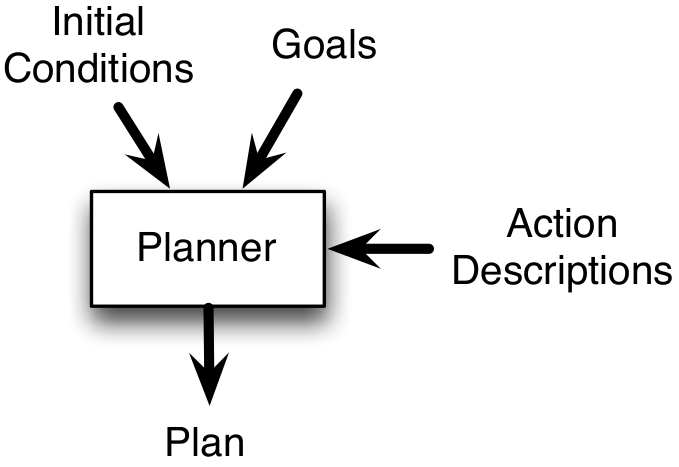
\includegraphics[height=0.5\textheight]{david-traditional}

\medskip

{\footnotesize (Figure from [\cite{smith:aaai-12}])}

\end{frame}


\begin{frame}{A Typical Reality: Interactive Decision Making}

\centering

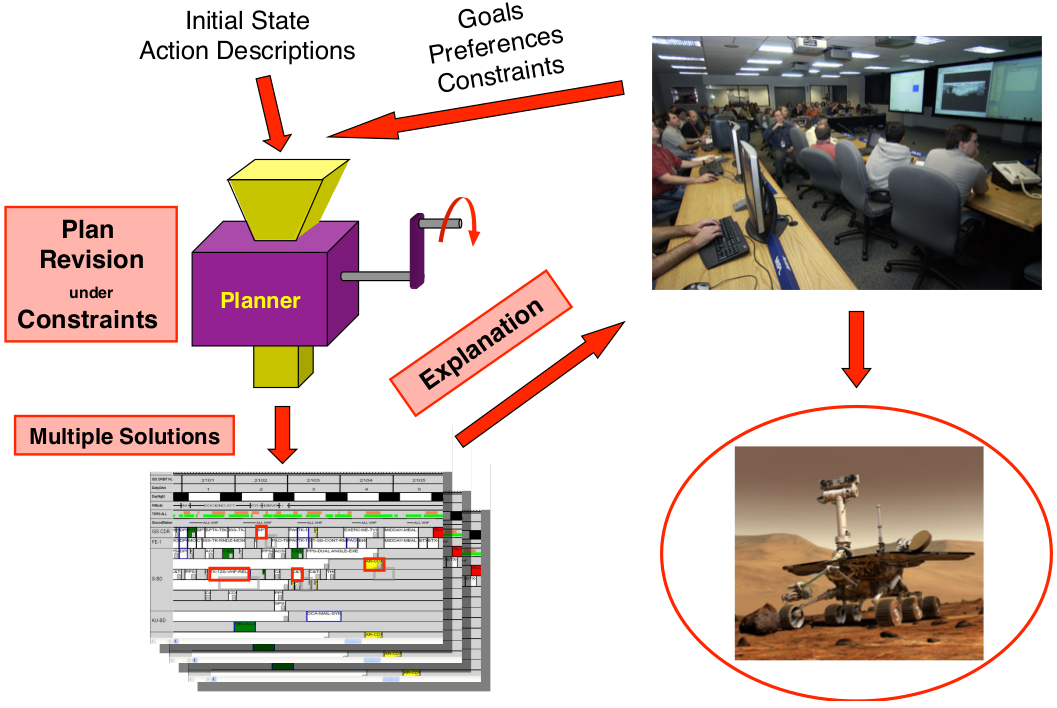
\includegraphics[height=0.75\textheight]{david-process}

\medskip

{\footnotesize (Figure from [\cite{smith:aaai-12}])}

\end{frame}


\begin{frame}{The Problem}

\centering

\begin{tikzpicture}
\node[] (human) at (-3,-2.3) {\huge Human};
\node[] (ai) at (2.8,-2.3) {\huge AI};

\visible<1|handout:0>{
\node[] (i1) at (0,0) {
\includegraphics[scale=0.25]{part2-intro1.png}};
}

\visible<2|handout:0>{
\node[] (i2) at (-0.28,0.85) {
\includegraphics[scale=0.25]{part2-intro2.png}};
\node[] (solution) at (-3.3,3.5) {\large Solution};
\node[] (task) at (-1.6,2.5) {\large Task};
}

\visible<3|handout:0>{
\node[] (i3) at (0,0.85) {
\includegraphics[scale=0.25]{part2-intro3.png}};
\node[] (solution) at (-3.3,3.5) {\large Solution};
\node[] (task) at (-1.6,2.5) {\large Task};
\node[] (plan) at (4.0,3.2) {\large Plan};
}

\visible<4|handout:0>{
\node[] (i4) at (0.28,0.57) {
\includegraphics[scale=0.25]{part2-intro4.png}};
\node[align=center] (why) at (-2.0,3.4) {Why this plan and \\not another plan?};
\node[] (plan) at (4.0,3.2) {\large Plan};
}

\visible<5|handout:1>{
\node[] (i5) at (-0.285,0.29) {
\includegraphics[scale=0.25]{part2-intro5.png}};
\node[align=center] (why) at (-2.0,3.4) {Why this plan and \\not another plan?};
}

\visible<6|handout:0>{
\node[] (i6) at (0,0.57) {
\includegraphics[scale=0.25]{part2-intro6.png}};
}
\end{tikzpicture}

\medskip

\end{frame}


\begin{frame}{Our Approach: Plan-Property Dependencies}

\centering

\begin{tikzpicture}
\node[] (human) at (-3,-2.3) {\huge Human};
\node[] (ai) at (2.8,-2.3) {\huge AI};

\visible<1|handout:0>{
\node[] (i3) at (0,0.85) {
\includegraphics[scale=0.25]{part2-intro3.png}};
\node[] (solution) at (-3.3,3.5) {\large Solution};
\node[] (task) at (-1.6,2.5) {\large Task};
\node[] (plan) at (4.0,3.2) {\large Plan};
}

\visible<2|handout:0>{
\node[] (i4) at (0.28,0.57) {
\includegraphics[scale=0.25]{part2-intro4.png}};
\node[align=center] (why) at (-2.0,3.4) {Why this plan and \\not another plan?};
\node[] (plan) at (4.0,3.2) {\large Plan};
}

\visible<3|handout:0>{
\node[] (i4) at (0.28,0.57) {
\includegraphics[scale=0.25]{part2-intro4.png}};
\node[align=center] (why) at (-2.0,3.4) {Why a plan with \textcolor{red}{property A},\\ not one with \textcolor{dkgreen}{property B?}};
\node[] (plan) at (4.0,3.2) {\large Plan};
}

\visible<4|handout:1>{
\node[] (i5) at (-0.285,0.29) {
\includegraphics[scale=0.333]{part2-intro5b.png}};
\node[align=center] (why) at (-2.0,3.4) {Why a plan with \textcolor{red}{property A},\\ not one with \textcolor{dkgreen}{property B?}};
\node[align=center] (dependency) at (3.5,3.4) {Because all plans\\ with \textcolor{dkgreen}{property B}\\ have \textcolor{red}{property C!}};
}

\visible<5|handout:0>{
\node[] (i6) at (0,0.57) {
\includegraphics[scale=0.333]{part2-intro6b.png}};
\node[align=center] (dependency) at (3.5,3.4) {Because all plans\\ with \textcolor{dkgreen}{property B}\\ have \textcolor{red}{property C!}};
}
\end{tikzpicture}

\medskip

\end{frame}


\begin{frame}{Our Approach in Interactive AI Planning}

\centering

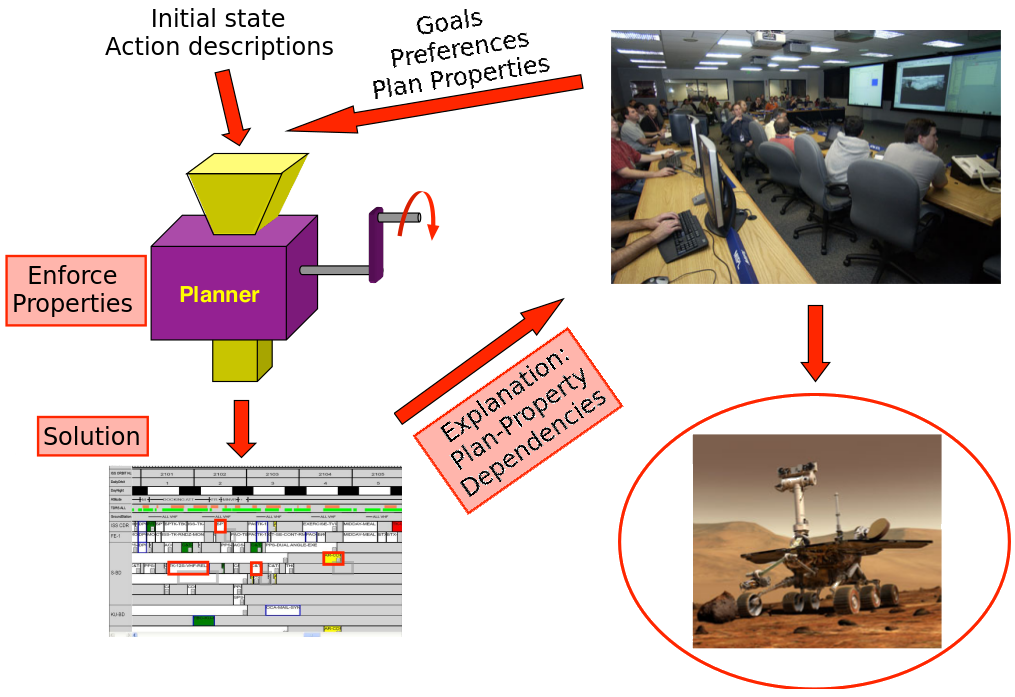
\includegraphics[height=0.75\textheight]{david-process-adapted}

\medskip

{\footnotesize (Figure adapted from [\cite{smith:aaai-12}])}

\end{frame}


\begin{frame}{Oversubscription Planning}

\begin{block}{Oversubscription Planning \hfill {\footnotesize [\cite{smith:icaps-04,domshlak:mirkis:jair-15}]}}
An \defined{OSP task} is a tuple \textred{$\task =
(\vars,\allowbreak\acts,\allowbreak\cost,\allowbreak\init,\allowbreak\goalhard,\allowbreak\goalsoft,\allowbreak\costbound)$}:
\begin{itemize}
\item \vars\ Variables, \acts\ Actions, \cost\ action-cost function, 
\init\ initial state;
\item \goalhard\ \defined{hard} goal;
\item \goalsoft\ \defined{soft} goal;
\item $\costbound \in \reals^+_0$ \defined{cost bound}.
\end{itemize}
As before: outcome state of applicable action sequence $\plan$ denoted
$s\apply{\plan}$. \plan\ is a \defined{plan} if
cost \textred{$\leq \costbound$ and
$\goalhard \subseteq \init\apply{\plan}$}.
%
%% An \defined{oversubscription planning (OSP) task} is a tuple $\task =
%% (\vars,\allowbreak\acts,\allowbreak\cost,\allowbreak\init,\allowbreak\goalhard,\allowbreak\goalsoft,\allowbreak\costbound)$
%% like an FDR task but with two goals -- the \defined{hard} goal
%% \goalhard\ and the \defined{soft} goal \goalsoft, assumed to be
%% defined on disjoint sets of variables -- as well as an additional
%% \defined{cost bound} $\costbound \in \reals^+_0$. A \defined{plan} is
%% an action sequence \plan\ whose summed-up cost is $\leq \costbound$
%% and where $\goalhard \subseteq \init\apply{\plan}$.
%
\end{block}

\bigskip \pause

\textbf{Plan Quality:} Usually additive soft-goal rewards. \pause Here:

\begin{itemize}
\item User preferences hard to specify/elicitate. Iterative planning instead.
\item Plan-property dependencies to support that process.
\end{itemize}

\medskip

\end{frame}


\begin{frame}{(Toy) Example: Mars Rover}

\centering

\vspace{-0.2cm}

\begin{tikzpicture}
\visible<1->{
\node[] (r1) at (1.5,2) {
\includegraphics[scale=0.07]{rover2.png}};
\node[] (b1) at (0.5,2.5) {
\includegraphics[scale=0.07]{battery.png}};
\node[] (r2) at (-5,-2.5) {
\includegraphics[scale=0.07]{rover1.png}};
\node[] (b2) at (-5,-3.5) {
\includegraphics[scale=0.07]{battery.png}};

\node[] (m) at (0,0) {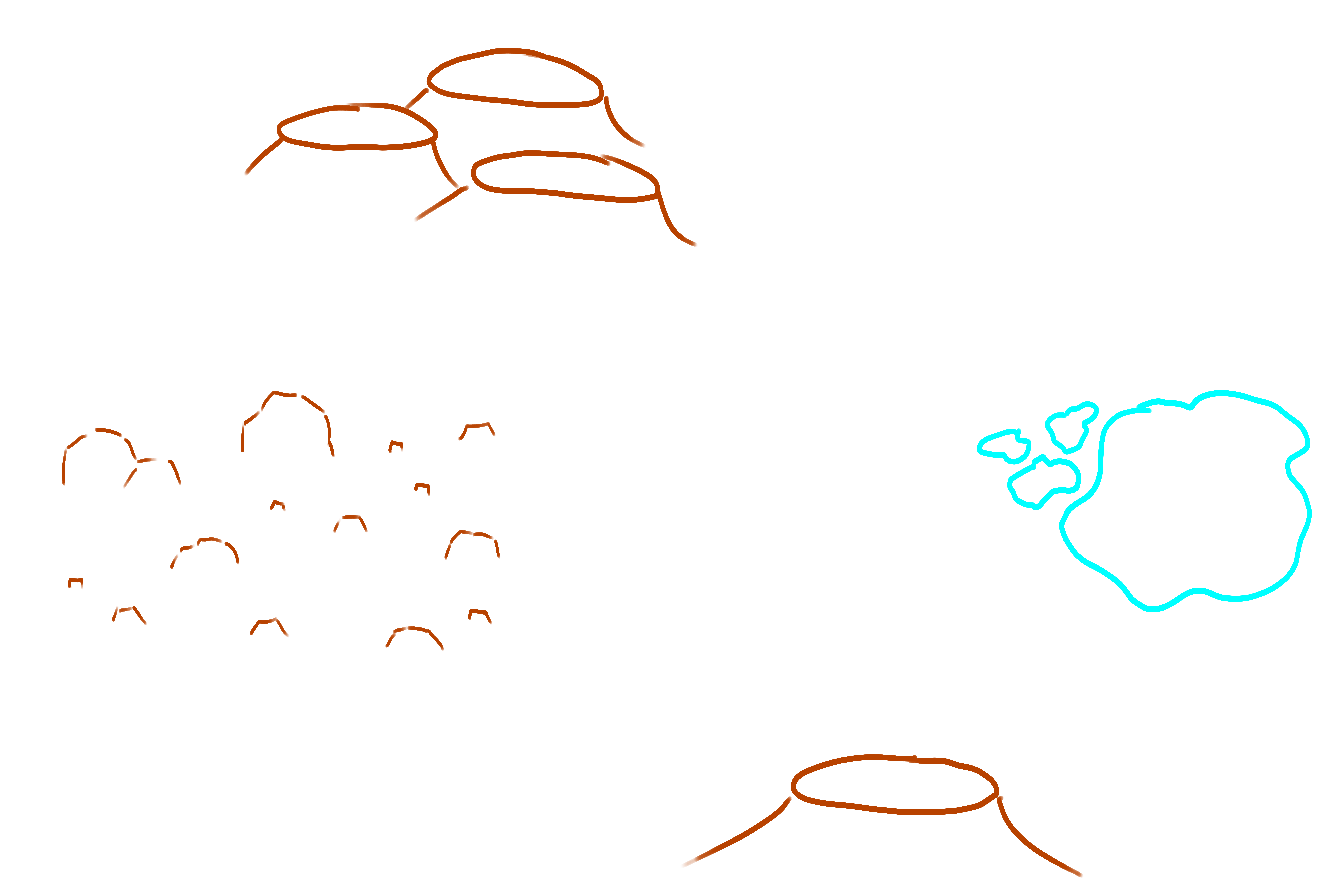
\includegraphics[scale=0.2]{mars.png}};
}

\visible<2->{
\node[] (g) at (-1.9,-4) {\Large \textbf{goal}:};
\node[] (i1) at (-0.5,-4) {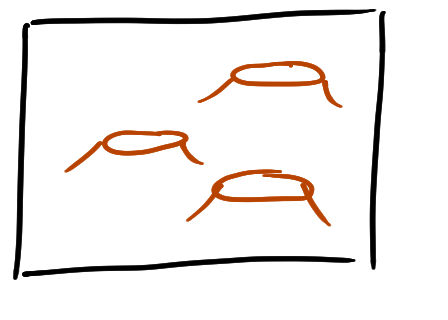
\includegraphics[scale=0.1]{rovergoal1.png}};
\node[] (i2) at (0.8,-4) {
\includegraphics[scale=0.1]{rovergoal2.png}};
\node[] (i3) at (2.5,-4) {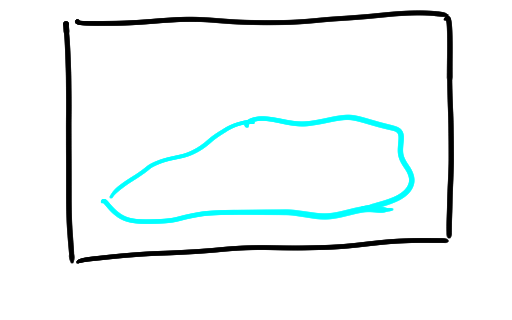
\includegraphics[scale=0.1]{rovergoal3.png}};
\node[] (i1) at (-0.5,-3.3) {$I_1$};
\node[] (i2) at (0.8,-3.4) {$I_2$};
\node[] (i3) at (2.5,-3.3) {$I_3$};
}

\visible<3->{
\node[draw, circle, inner sep=3pt] (l1) at (-3,-3) {$L_1$};
\node[draw, circle, inner sep=3pt] (l2) at (-2.1,1.3) {$L_2$};
\node[draw, circle, inner sep=3pt] (l3) at (-0.5,-1) {$L_3$};
\node[draw, circle, inner sep=3pt] (l4) at (3,2) {$L_4$};
\node[draw, circle, inner sep=3pt] (l5) at (1.8,0) {$L_5$};
\node[draw, circle, inner sep=3pt] (l6) at (3.2,-2.5) {$L_6$};

\draw[thick] (l1) to (l2);
\draw[thick] (l1) to (l3);
\draw[thick] (l2) to (l3);
\draw[thick] (l3) to (l5);
\draw[thick] (l4) to (l5);
\draw[thick] (l4) to (l6);
\draw[thick] (l5) to (l6);
}

\visible<4->{
\node[align=left] (actions) at (-5.5,2) {
%\Large \textbf{actions}:\\
%\vspace*{0.2cm}
\begin{varwidth}{4.0cm}
\begin{itemize}
\item $drive(R_i,L_x,L_y)$
\item $takeImage(I_x,R_y)$
\end{itemize}
\end{varwidth}
};
}
\end{tikzpicture}
	
\end{frame}


\begin{frame}{Mars Rover OSP}

\centering

\begin{tikzpicture}
\node[] (el) at (0,0) {\Large energy limit};
\node[] (el) at (3,0) {
\includegraphics[scale=0.2]{battery-low.png}};
\end{tikzpicture}

\bigskip \medskip

\visible<2>{
\begin{tabular}{c|c|c}
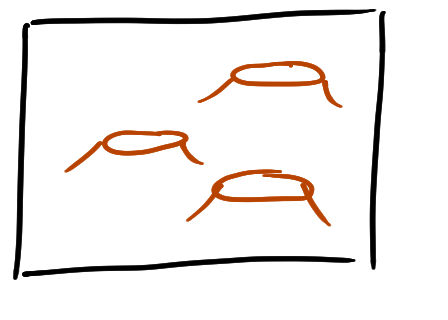
\includegraphics[scale=0.15]{rovergoal1.png} &

\includegraphics[scale=0.15]{rovergoal2.png} &
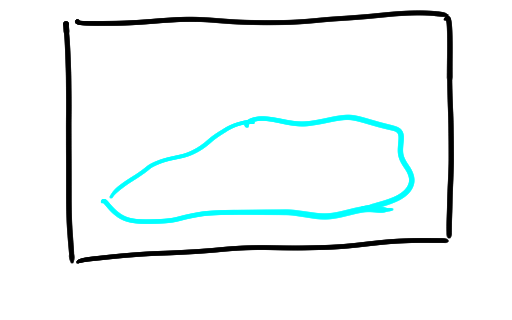
\includegraphics[scale=0.15]{rovergoal3.png} \\\hline


\includegraphics[scale=0.1]{yes.png} &

\includegraphics[scale=0.1]{no.png} &

\includegraphics[scale=0.1]{yes.png} \\

\end{tabular}
}

\medskip

\end{frame}


\begin{frame}{Our Problem in Mars Rover}

\centering

\begin{tikzpicture}
\node[] (task) at (-6,1) {
\begin{tikzpicture}
\node[] (p) at (0,2) {\textbf{Planning Task}};
\node[] (r1) at (0,-0.3) {
\includegraphics[scale=0.06]{rover1.png}};
\node[] (r2) at (1.5,-0.3) {
\includegraphics[scale=0.06]{rover2.png}};
\node[] (i1) at (-0.5,1) {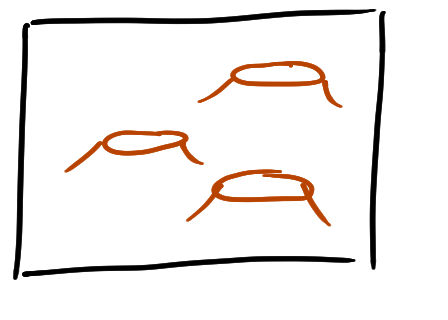
\includegraphics[scale=0.07]{rovergoal1.png}};
\node[] (i2) at (0.5,1) {
\includegraphics[scale=0.07]{rovergoal2.png}};
\node[] (i3) at (1.7,1) {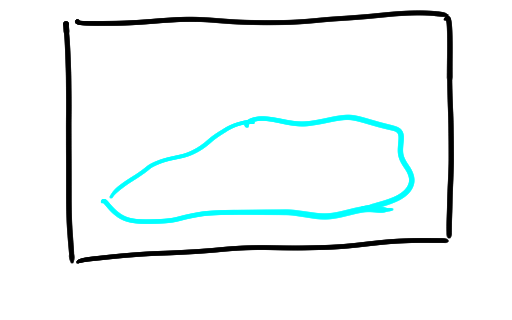
\includegraphics[scale=0.07]{rovergoal3.png}};
\end{tikzpicture}
};

\visible<2->{
\node[] (p) at (0,2.5) {\textbf{Plan}};
\node[draw, align=left, fill=white] (p1) at (0,0.9) {
$drive(R_1,L_1,L2)$\\
$takeImage(I_1, R_1)$\\
$drive(R_2,L_4,L_5)$\\
$takeImage(I_3, R_2)$
};
}

\visible<3->{
\node[fill=white] (p1) at (-0.0,-1.65) {
\begin{tabular}{c|c|c}
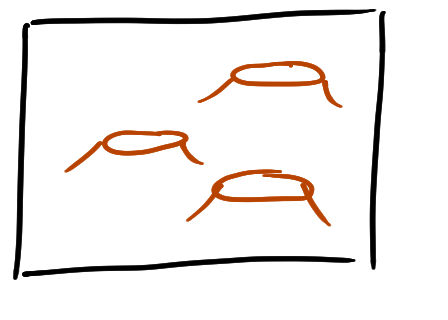
\includegraphics[scale=0.07]{rovergoal1.png} &

\includegraphics[scale=0.07]{rovergoal2.png} &
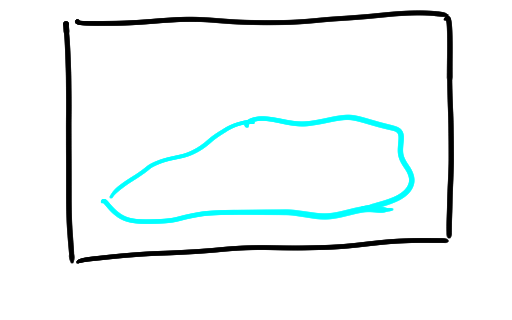
\includegraphics[scale=0.07]{rovergoal3.png} \\\hline


\includegraphics[scale=0.05]{yes.png} &

\includegraphics[scale=0.05]{no.png} &

\includegraphics[scale=0.05]{yes.png} \\

\end{tabular}
};
}

\visible<4>{
\node[] (hw) at (-4.0,-2.5) {
\includegraphics[scale=0.2]{human-why.png}};
}
\end{tikzpicture}
	
\end{frame}



%%%%%%%%%%%%%%%%%%%%%%%%%%%%%%%%%%%%%%%%%%%%%%%%%%%%%%%%%%%%%%%%%%%%%%%%%%%%%%%%%
%%%%%%%%%%%%%%%%%%%%%%%%%%%%%%%%%%%%%%%%%%%%%%%%%%%%%%%%%%%%%%%%%%%%%%%%%%%%%%%%%
%%%%%%%%%%%%%%%%%%%%%%%%%%%%%%%%%%%%%%%%%%%%%%%%%%%%%%%%%%%%%%%%%%%%%%%%%%%%%%%%%
%%% Explanation Framework
%
%%% Timing: XX min

\section[Framework]{Explanation Framework}
\subsection*{}

\begin{frame}{}

\end{frame}



%%%%%%%%%%%%%%%%%%%%%%%%%%%%%%%%%%%%%%%%%%%%%%%%%%%%%%%%%%%%%%%%%%%%%%%%%%%%%%%%%
%%%%%%%%%%%%%%%%%%%%%%%%%%%%%%%%%%%%%%%%%%%%%%%%%%%%%%%%%%%%%%%%%%%%%%%%%%%%%%%%%
%%%%%%%%%%%%%%%%%%%%%%%%%%%%%%%%%%%%%%%%%%%%%%%%%%%%%%%%%%%%%%%%%%%%%%%%%%%%%%%%%
%%% Computing Explanations
%
%%% Timing: XX min

\section[Computing]{Computing Explanations}
\subsection*{}

\begin{frame}{}

\end{frame}



%%%%%%%%%%%%%%%%%%%%%%%%%%%%%%%%%%%%%%%%%%%%%%%%%%%%%%%%%%%%%%%%%%%%%%%%%%%%%%%%%
%%%%%%%%%%%%%%%%%%%%%%%%%%%%%%%%%%%%%%%%%%%%%%%%%%%%%%%%%%%%%%%%%%%%%%%%%%%%%%%%%
%%%%%%%%%%%%%%%%%%%%%%%%%%%%%%%%%%%%%%%%%%%%%%%%%%%%%%%%%%%%%%%%%%%%%%%%%%%%%%%%%
%%% Compilations
%
%%% Timing: XX min

\section[Compilations]{Compilations}
\subsection*{}

\begin{frame}{}

\end{frame}



%%%%%%%%%%%%%%%%%%%%%%%%%%%%%%%%%%%%%%%%%%%%%%%%%%%%%%%%%%%%%%%%%%%%%%%%%%%%%%%%%
%%%%%%%%%%%%%%%%%%%%%%%%%%%%%%%%%%%%%%%%%%%%%%%%%%%%%%%%%%%%%%%%%%%%%%%%%%%%%%%%%
%%%%%%%%%%%%%%%%%%%%%%%%%%%%%%%%%%%%%%%%%%%%%%%%%%%%%%%%%%%%%%%%%%%%%%%%%%%%%%%%%
%%% Current Results
%
%%% Timing: XX min

\section[Results]{Current Results}
\subsection*{}

\begin{frame}{}

\end{frame}



%%%%%%%%%%%%%%%%%%%%%%%%%%%%%%%%%%%%%%%%%%%%%%%%%%%%%%%%%%%%%%%%%%%%%%%%%%%%%%%%%
%%%%%%%%%%%%%%%%%%%%%%%%%%%%%%%%%%%%%%%%%%%%%%%%%%%%%%%%%%%%%%%%%%%%%%%%%%%%%%%%%
%%%%%%%%%%%%%%%%%%%%%%%%%%%%%%%%%%%%%%%%%%%%%%%%%%%%%%%%%%%%%%%%%%%%%%%%%%%%%%%%%
%%% NoGood Learning in State Space
%
%%% Timing: XX min

\section[NoGood Learning]{NoGood Learning in State Space}
\subsection*{}

\begin{frame}{}

\end{frame}



%%%%%%%%%%%%%%%%%%%%%%%%%%%%%%%%%%%%%%%%%%%%%%%%%%%%%%%%%%%%%%%%%%%%%%%%%%%%%%%%%
%%%%%%%%%%%%%%%%%%%%%%%%%%%%%%%%%%%%%%%%%%%%%%%%%%%%%%%%%%%%%%%%%%%%%%%%%%%%%%%%%
%%%%%%%%%%%%%%%%%%%%%%%%%%%%%%%%%%%%%%%%%%%%%%%%%%%%%%%%%%%%%%%%%%%%%%%%%%%%%%%%%
%%% Last Slide & References

\section*{}

\begin{frame}{Last Slide}

{\centering

Thanks for your attention. Questions?

}

\end{frame}

\section*{}

\begin{frame}[allowframebreaks]{References}
\footnotesize
\bibliographystyle{named}
\bibliography{abbreviations,biblio,crossref}
\end{frame}



%%%%%%%%%%%%%%%%%%%%%%%%%%%%%%%%%%%%%%%%%%%%%%%%%%%%%%%%%%%%%%%%%%%
%%%%%%%%%%%%%%%%%%%%%%%%%%%%%%%%%%%%%%%%%%%%%%%%%%%%%%%%%%%%%%%%%%%
%%%%%%%%%%%%%%%%%%%%%%%%%%%%%%%%%%%%%%%%%%%%%%%%%%%%%%%%%%%%%%%%%%%
%%% BACKUP SLIDES


\end{document}
